\documentclass{report}
\usepackage{fancyvrb}
\usepackage{graphicx}
\usepackage{float}
\usepackage
[
a4paper,% other options: a3paper, a5paper, etc
left=3cm,
right=1cm,
top=3cm,
bottom=4cm,
% use vmargin=2cm to make vertical margins equal to 2cm.
% us  hmargin=3cm to make horizontal margins equal to 3cm.
% use margin=3cm to make all margins  equal to 3cm.
]
{geometry}
\author{Mehmet Hakan Satman (PhD.)}
\title{Tkinter Tutorial for Python}

\setcounter{chapter}{1}

\begin{document}
	\maketitle
	\tableofcontents
	
\section{Initials}
Importing the required package, \texttt{tkinter}:
\begin{Verbatim}[frame = single]
	from tkinter import *
\end{Verbatim}
This use of  \texttt{import} imports the package content and registers the function names into the global namespace.

\begin{Verbatim}[frame = single]
from tkinter import *

root = Tk()

win = Frame(root)

win.pack()

root.mainloop()
\end{Verbatim}

\begin{figure}[H]
	\centering
	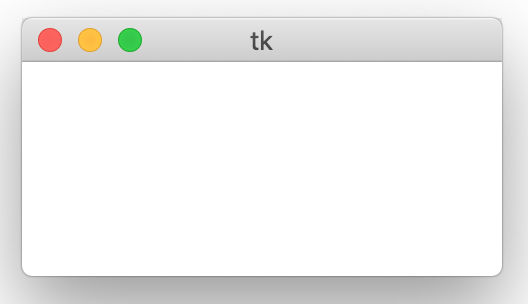
\includegraphics{images/emptyframe.png}
\end{figure}


\pagebreak
\section{Hello, World!}
\begin{Verbatim}[frame = single]
from tkinter import *

root = Tk()

win = Frame(root)

lab = Label(win, text = "Hello, world! from Python tkinter", fg="red", bg="white")

lab.grid(column = 1, row = 1)

win.pack()

root.mainloop()
\end{Verbatim}

\begin{figure}[H]
	\centering
	
\includegraphics{images/helloworld.png}
\end{figure}


\pagebreak
\section{The 'Click me!' Button}

\begin{Verbatim}[frame = single]
	from tkinter import *
	
	root = Tk()
	
	win = Frame(root)
	
	lab = Label(win, text = "Hello, world! from Python tkinter", fg="red", bg="white")
	
	mybutton = Button(win, text = "Click me!")
	
	lab.grid(column = 1, row = 1)
	mybutton.grid(column = 1, row = 2)
	
	win.pack()
	
	root.mainloop()
\end{Verbatim}


\begin{figure}[H]
	\centering
	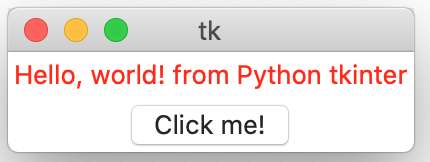
\includegraphics{images/clickme.png}
\end{figure}




\pagebreak
\section{Button with event handling}

\begin{Verbatim}[frame = single]
from tkinter import *
from tkinter import messagebox

def handleClick():
    messagebox.showinfo(title = "info", message = "You clicked!")

root = Tk()
win = Frame(root)

lab = Label(win, text = "Hello, world! from Python tkinter", fg="red", bg="white")
mybutton = Button(win, text = "Click me!", command = handleClick)

lab.grid(column = 1, row = 1)
mybutton.grid(column = 1, row = 2)

win.pack()

root.mainloop()
\end{Verbatim}


\begin{figure}[H]
	\centering
	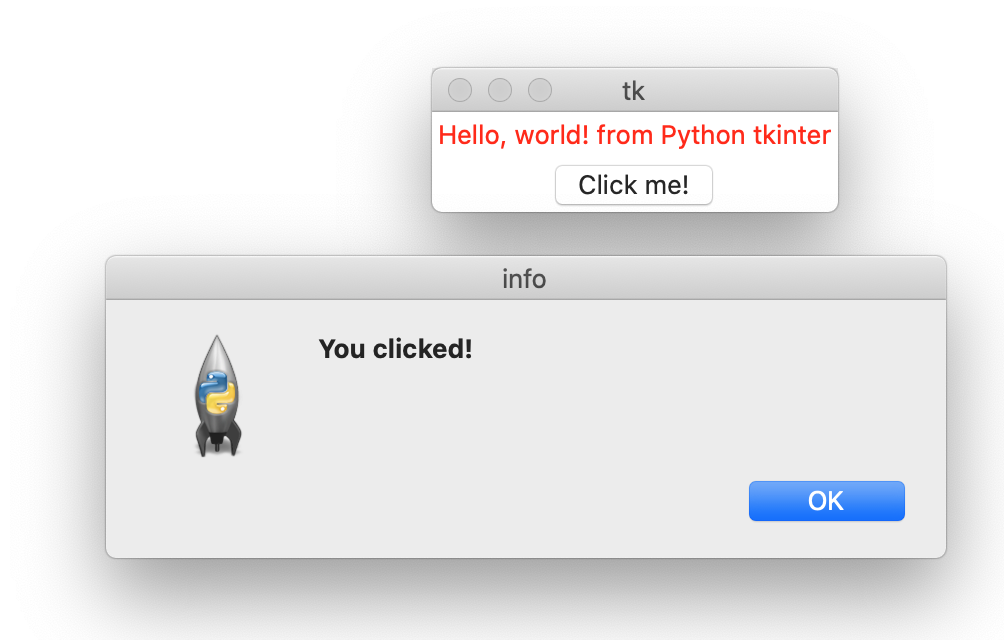
\includegraphics{images/clickmewithevents.png}
\end{figure}



\pagebreak
\section{The Textbox}

\begin{Verbatim}[frame = single]
from tkinter import *
from tkinter import messagebox

def handleClick():
    messagebox.showinfo(title = "info", message = "Hello " + varName.get())

root = Tk()
varName = StringVar()

win = Frame(root)
lab = Label(win, text = "Please enter your name:", fg="red", bg="white")
enterybox = Entry(win, fg="black", bg="white", textvariable = varName)
mybutton = Button(win, text = "Click me!", command = handleClick)

lab.grid(column = 1, row = 1)
enterybox.grid(column = 1, row = 2)
mybutton.grid(column = 1, row = 3)

win.pack()

root.mainloop()
\end{Verbatim}


\begin{figure}[H]
	\centering
	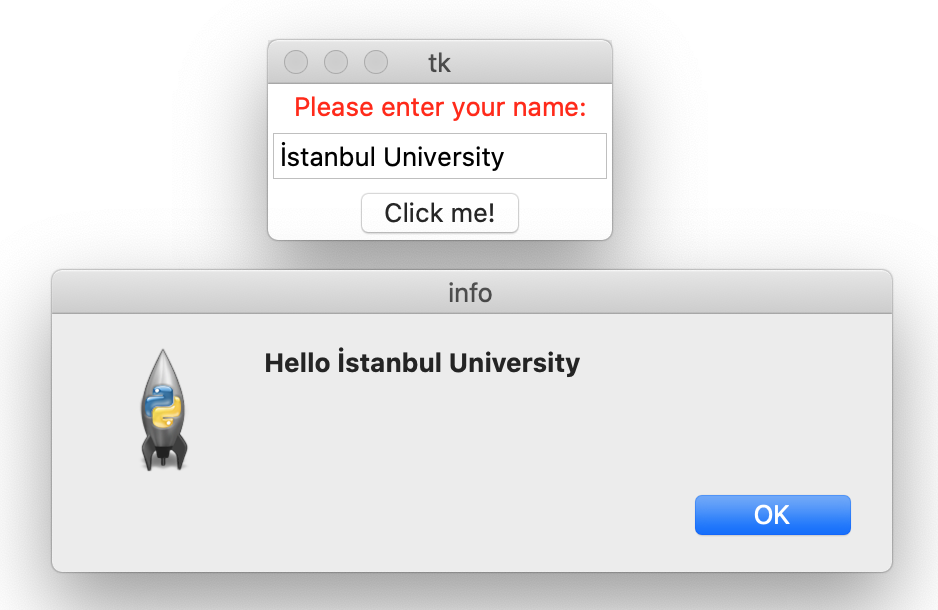
\includegraphics{images/textbox.png}
\end{figure}



\pagebreak
\section{Checkbox}

\begin{Verbatim}
from tkinter import *
from tkinter import messagebox

def buttonOnClick():
    strMessage = "The user: "
    if(abilityEng.get() == 1):
        strMessage += "Speaks english"
    if(abilityAnalysis.get() == 1):
        strMessage += "\nCan analysis data"
    messagebox.showinfo(title = "", message = strMessage)

root = Tk()

win = Frame(root)

abilityEng = IntVar()
abilityAnalysis = IntVar()

check1 = Checkbutton(master = win, text = "Speaks English?", var = abilityEng)
check2 = Checkbutton(master = win, text = "Can analysis data?", var = abilityAnalysis)
button = Button(master = win, text = "Submit", command = buttonOnClick)

check1.grid(row = 1, column = 1)
check2.grid(row = 1, column = 2)
button.grid(row = 2, columnspan = 2)
win.pack()

root.mainloop()
\end{Verbatim}

\begin{figure}[H]
	\centering
	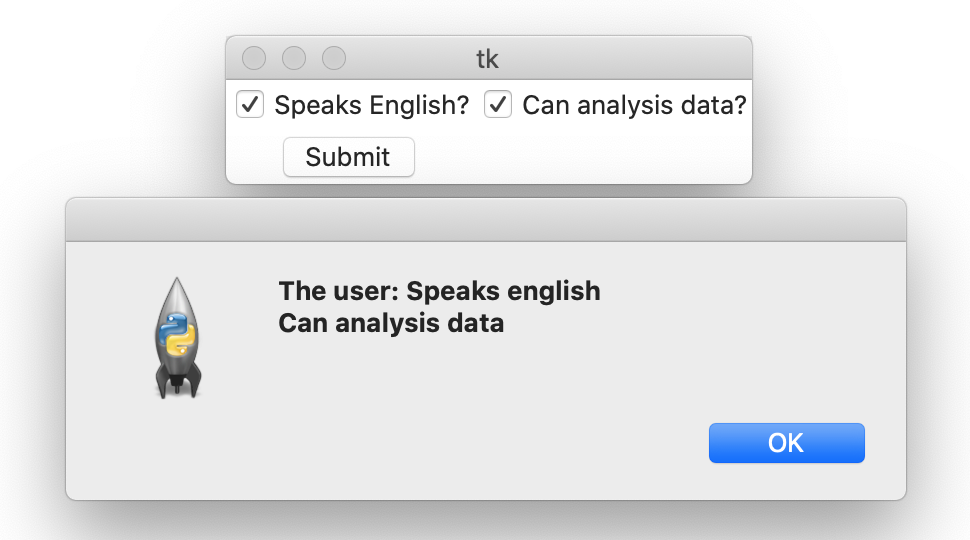
\includegraphics{images/checkbox.png}
\end{figure}


\pagebreak
\section{RadioButton}
\begin{Verbatim}[frame = single]
from tkinter import *
from tkinter import messagebox

def handleOption():
    messagebox.showinfo(message = "You select " + language.get())

root = Tk()

win = Frame(root)

language = StringVar()

radio1 = Radiobutton(master = win, text = "R", var = language, 
value = "R", command = handleOption)

radio2 = Radiobutton(master = win, text = "Python", var = language, 
value = "Python", command = handleOption)

radio3 = Radiobutton(master = win, text = "Julia", var = language, 
value = "Julia", command = handleOption)

radio1.grid(row = 1, column = 1)
radio2.grid(row = 1, column = 2)
radio3.grid(row = 1, column = 3)

win.pack()

root.mainloop()
\end{Verbatim}


\begin{figure}[H]
	\centering
	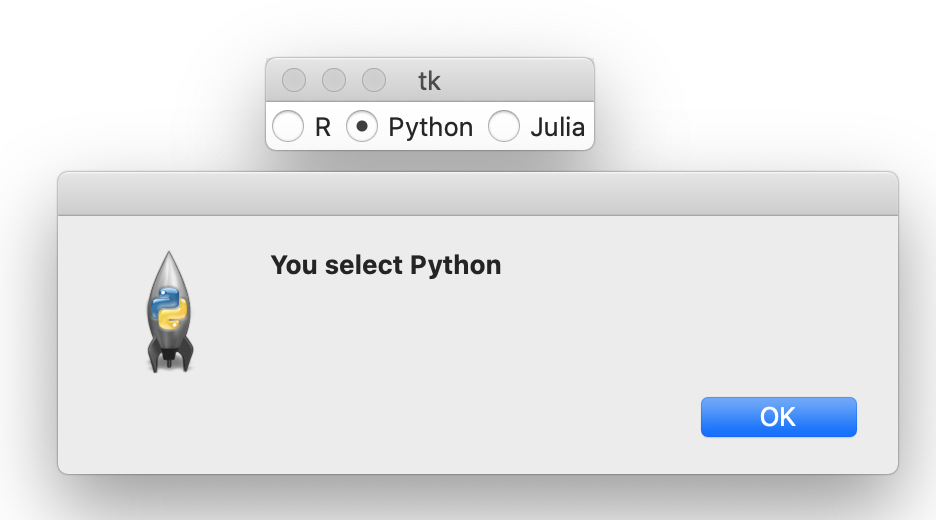
\includegraphics{images/radiobutton.png}
\end{figure}



\section{ListBox}

\begin{Verbatim}[frame = single]
from tkinter import *
from tkinter import messagebox

def handleButton():
messagebox.showinfo(message = "You select " + mylist.selection_get())

root = Tk()

win = Frame(root)

mylist = Listbox(master = win)
mylist.insert(1, "Econometrics")
mylist.insert(2, "Mathematics")
mylist.insert(3, "Macro Economics")

button = Button(master = win, text = "Select", command = handleButton)

mylist.grid(row = 1, column = 1)
button.grid(row = 2, column = 1)
win.pack()

root.mainloop()
\end{Verbatim}

\begin{figure}[H]
	\centering
	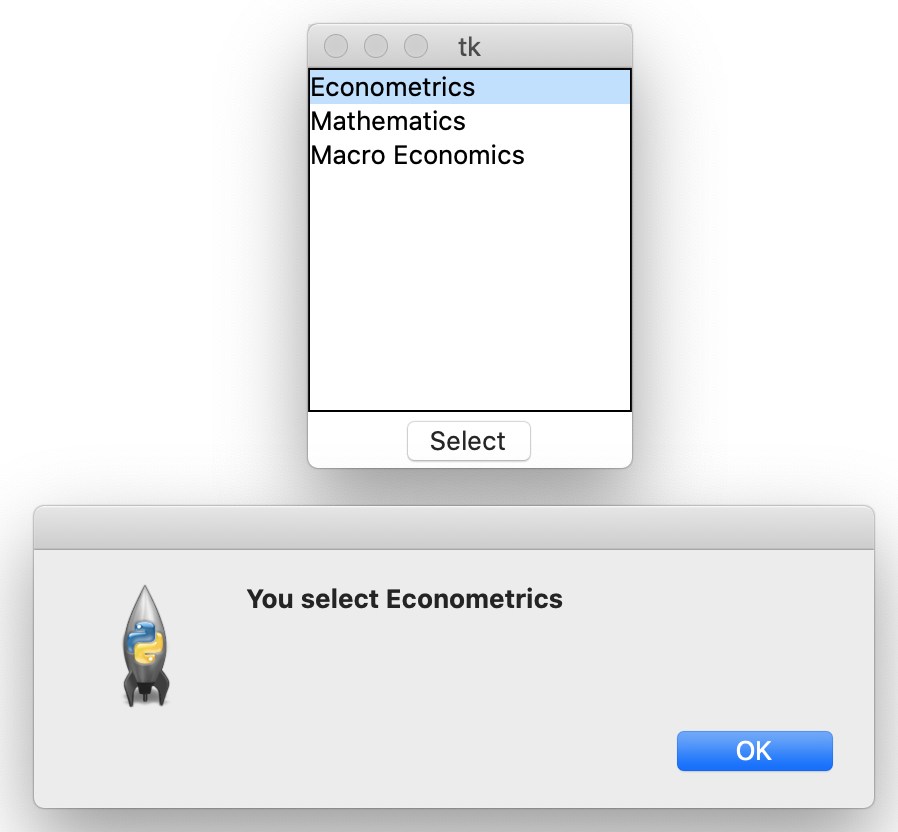
\includegraphics{images/listbox.png}
\end{figure}


\end{document}